\documentclass[12pt]{beamer}
\setbeamertemplate{navigation symbols}{}
\usetheme{Copenhagen}
\usepackage{listings}
\usepackage{xcolor}
\usepackage{graphicx}
\usepackage{hyperref}
\usepackage{multicol}
\graphicspath{ {imagenes/} }

\definecolor{codegreen}{rgb}{0,0.6,0}
\definecolor{codegray}{rgb}{0.5,0.5,0.5}
\definecolor{codepurple}{rgb}{0.58,0,0.82}
\definecolor{backcolour}{rgb}{0.95,0.95,0.92}

\lstdefinestyle{mystyle}{
    language=c++,
    backgroundcolor=\color{backcolour},   
    commentstyle=\color{codegreen},
    keywordstyle=\color{magenta},
    numberstyle=\tiny\color{codegray},
    stringstyle=\color{codepurple},
    basicstyle=\ttfamily\footnotesize,
    breakatwhitespace=false,         
    breaklines=true,                 
    captionpos=b,                    
    keepspaces=true,                 
    numbers=left,                    
    numbersep=5pt,                  
    showspaces=false,                
    showstringspaces=false,
    showtabs=false,                  
    tabsize=2
}

\lstset{style=mystyle}

\title{Arreglos en C++}
\subtitle{Matrices}
\author{Tomás Peiretti}
\date{}

\begin{document}

\maketitle

\begin{frame}[fragile]{Arreglos multidimensionales}
    Los arreglos multidimensionales se pueden definir como \alert{arreglos de arreglos}. En AEDD usaremos arreglos bidimensionales, a los que llamaremos \alert{matrices} para resolver problemas.

    \smallskip

\begin{lstlisting}[basicstyle=\tiny]
int main() {
    char arreglo[100]; //el arreglo que conociamos hasta el momento
    int matriz[3][10]; //un arreglo bidimensional (matriz, arreglo de arreglos)
    int miArr[10][10][5]; //un arreglo tridimensional (un arreglo de arreglos que contienen arreglos)
    bool arr[5][3][5][4][205]; //un arreglo de 5 dimensiones
}
\end{lstlisting}
    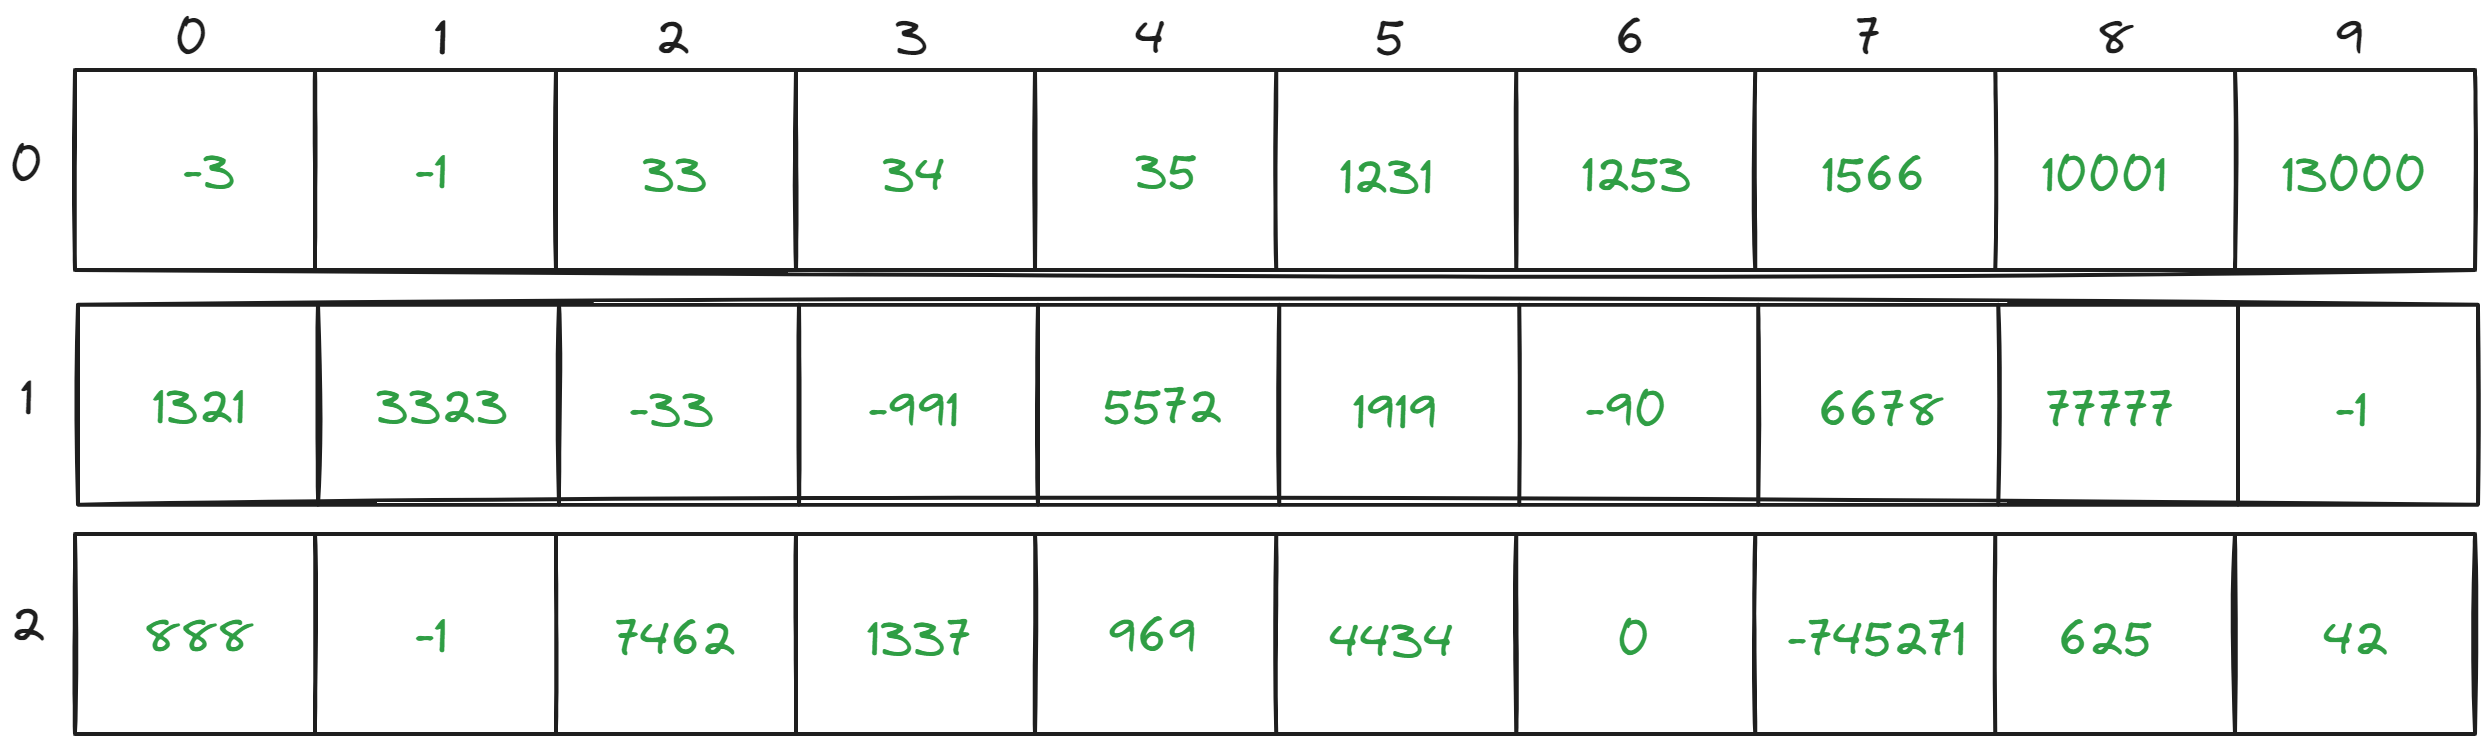
\includegraphics[width=\textwidth]{matriz.png}
\end{frame}

\begin{frame}{Arreglos multidimensionales}
    Para \alert{acceder a un elemento} de un arreglo multidimensional, al igual que con los arreglos normales, se debe indicar el indice correspondiente. Solo que esta vez, tendremos que \alert{indicar un índice para cada dimensión}:
    
    \smallskip
    
    Por ejemplo, si deseamos acceder al elemento de una matriz que se encuentra en la fila 1 y la columna 6 debemos hacer:
    \begin{center}
        matriz[\alert{0}][\alert{6}]
    \end{center}
    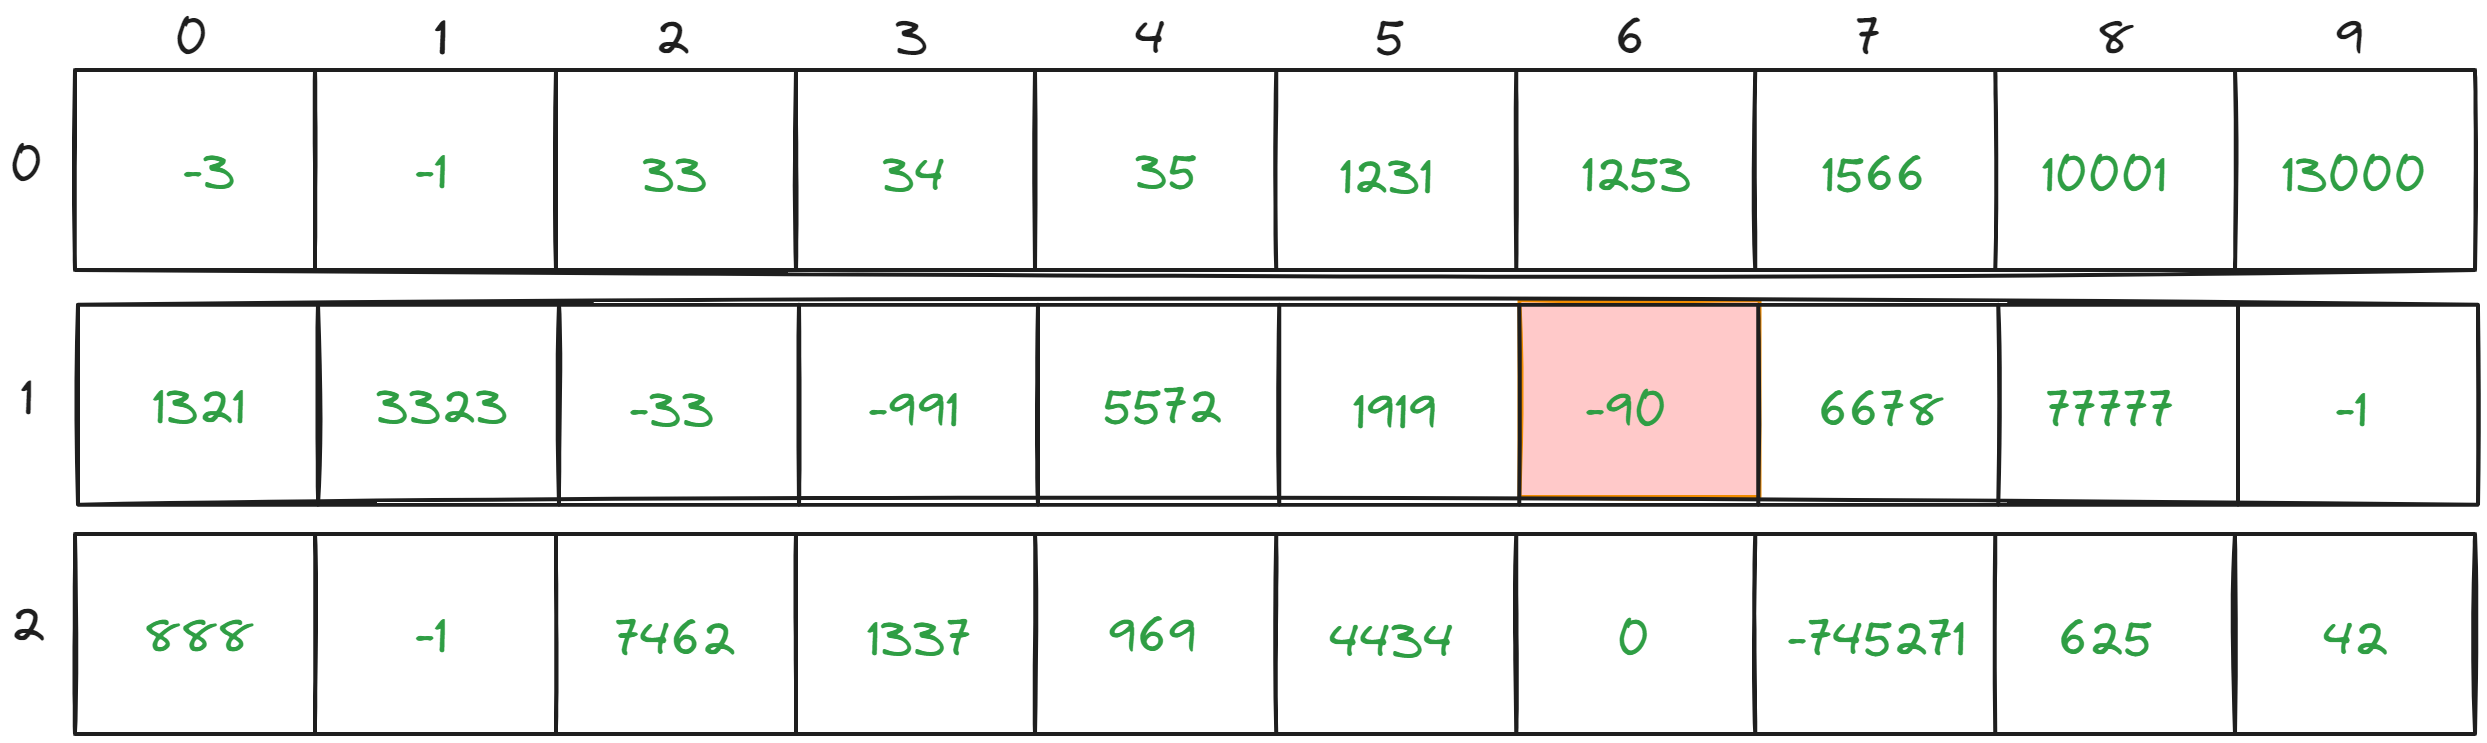
\includegraphics[width=\textwidth]{matriz_1_6.png}
\end{frame}

\begin{frame}[fragile]{Arreglos multidimensionales: funciones}
    Para pasar un arreglo multidimensional a una función, se debe indicar el tamaño de todas las dimensiones (excluyendo opcionalmente la primera). Sino, tendremos un error de compilación.

    \smallskip

\begin{lstlisting}[basicstyle=\tiny]
// ejemplo: miFuncion recibe una matriz como primer parametro,
// y ademas un arreglo de 4 dimensiones como segundo parametro
void miFuncion(char matriz[][10], int arr[][5][3][5]) {
    // ....
}        

int main() {
    char mat[30][10];
    int arregloMulti[10][5][3][5];
    
    miFuncion(mat, arregloMulti);
    return 0;
}
\end{lstlisting}

    \smallskip

    \begin{itemize}
        \item No olvidemos que los arreglos \alert{por defecto pasan por referencia}
    \end{itemize}
\end{frame}

\begin{frame}[fragile]{Arreglos multidimensionales: ejemplos}
\begin{lstlisting}[basicstyle=\tiny]
void imprimirMatriz(char mat[][20], int filas) {
    for (int i=0; i<filas; i++) {
        for (int j=0; j<20; j++) {
            cout << mat[i][j] << " ";
        }
        cout << endl;
    }
}

int sumaDiagonalPrincipal(int mat[][100], int tam) {
    int sum = 0;
    for (int i=0; i<tam; i++) {
        sum += mat[i][i];
    }
    return sum;
}

bool esTriangularSuperior(int mat[][100], int filas, int columnas) {
    bool esTriangularSup = true;
    if (filas != columnas) {
        esTriangularSup = false;
    } else {
        for (int i=1; i<filas; i++) {
            for (int j=0; j<i; j++) {
                if (mat[i][j] != 0)
                    esTriangularSup = false;
            }
        }
    }
    return esTriangularSup;
}
\end{lstlisting}
\end{frame}

\begin{frame}{Ejercicios}
    \begin{multicols}{2}
        \begin{itemize}
            \item \href{https://judge.beecrowd.com/es/problems/view/1181}{Beecrowd 1181}
            \item \href{https://judge.beecrowd.com/es/problems/view/1182}{Beecrowd 1182}
            \item \href{https://judge.beecrowd.com/es/problems/view/1183}{Beecrowd 1183}
            \item \href{https://judge.beecrowd.com/es/problems/view/1184}{Beecrowd 1184}
            \item \href{https://judge.beecrowd.com/es/problems/view/1185}{Beecrowd 1185}
            \item \href{https://judge.beecrowd.com/es/problems/view/1186}{Beecrowd 1186}
            \item \href{https://judge.beecrowd.com/es/problems/view/1187}{Beecrowd 1187}
            \item \href{https://judge.beecrowd.com/es/problems/view/1188}{Beecrowd 1188}
            \item \href{https://judge.beecrowd.com/es/problems/view/1189}{Beecrowd 1189}
            \item \href{https://judge.beecrowd.com/es/problems/view/1435}{Beecrowd 1435}
            \item \href{https://judge.beecrowd.com/es/problems/view/1478}{Beecrowd 1478}
            \item \href{https://judge.beecrowd.com/es/problems/view/1534}{Beecrowd 1534}
            \item \href{https://judge.beecrowd.com/es/problems/view/1557}{Beecrowd 1557}
            \item \href{https://judge.beecrowd.com/es/problems/view/1827}{Beecrowd 1827}
        \end{itemize}
    \end{multicols}
\end{frame}

\end{document}